\usepackage{geometry}
\geometry{a4paper, margin=1in}
\usepackage{graphicx}
\usepackage{listings}
\usepackage{xcolor}
\usepackage[utf8]{inputenc}

\lstset{
    basicstyle=\ttfamily\small,
    breaklines=true,
    frame=single,
    language=C++,
    keywordstyle=\color{blue},
    commentstyle=\color{green!50!black},
    stringstyle=\color{red}
}

\begin{document}

\title{Operating Systems Lab Assignment: Thread-Safe Data Structures}
\author{Bryce Coleman}
\date{October 21, 2025}
\maketitle

\section{Introduction}
This report documents the implementations and analyses for the thread-safe data structures lab assignment, covering thread-safe queue and stack implementations, Producer-Consumer and Undo-Redo use cases, and additional exercises.

\section{Exercise 1: Thread-Safe Queue and Stack}
\lstinputlisting[language=C++]{thread_safe_data_structures.cpp}

\textbf{Explanation}: Describe how mutexes ensure thread safety in ThreadSafeQueue and ThreadSafeStack. Explain the Producer-Consumer and Undo-Redo implementations.

\textbf{Analysis}: Discuss thread synchronization behavior and consumer termination logic.

\textbf{Screenshot}: Include a screenshot of compiling and running thread_safe_data_structures.cpp.
\begin{figure}[h]
    \centering
    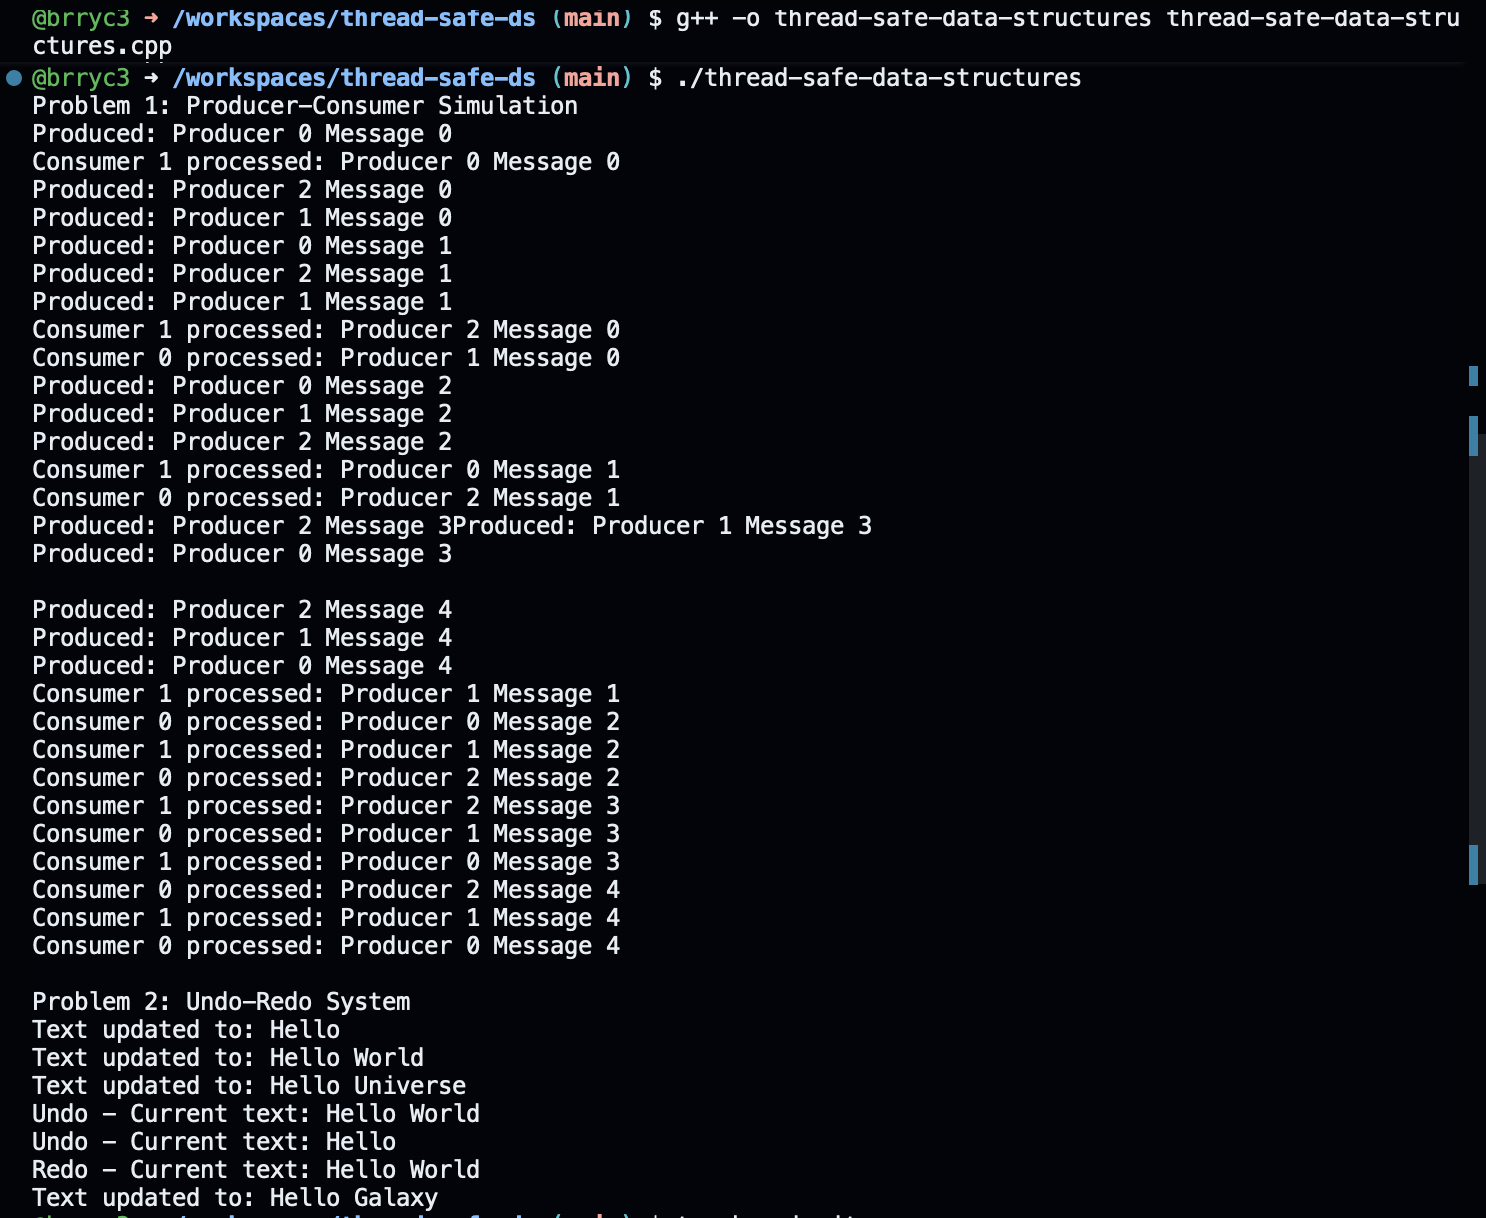
\includegraphics[width=\textwidth]{1_screenshot.png}
    \caption{Compilation and execution of thread_safe_data_structures.cpp}
\end{figure}

\section{Exercise 3: Thread-Safe Priority Queue}
\lstinputlisting[language=C++]{priority_queue.cpp}

\textbf{Explanation}: Describe how the priority queue maintains order and ensures thread safety.

\textbf{Analysis}: Analyze the behavior of concurrent pushes and pops.

\textbf{Screenshot}: Include a screenshot of compiling and running priority_queue.cpp.
\begin{figure}[h]
    \centering
    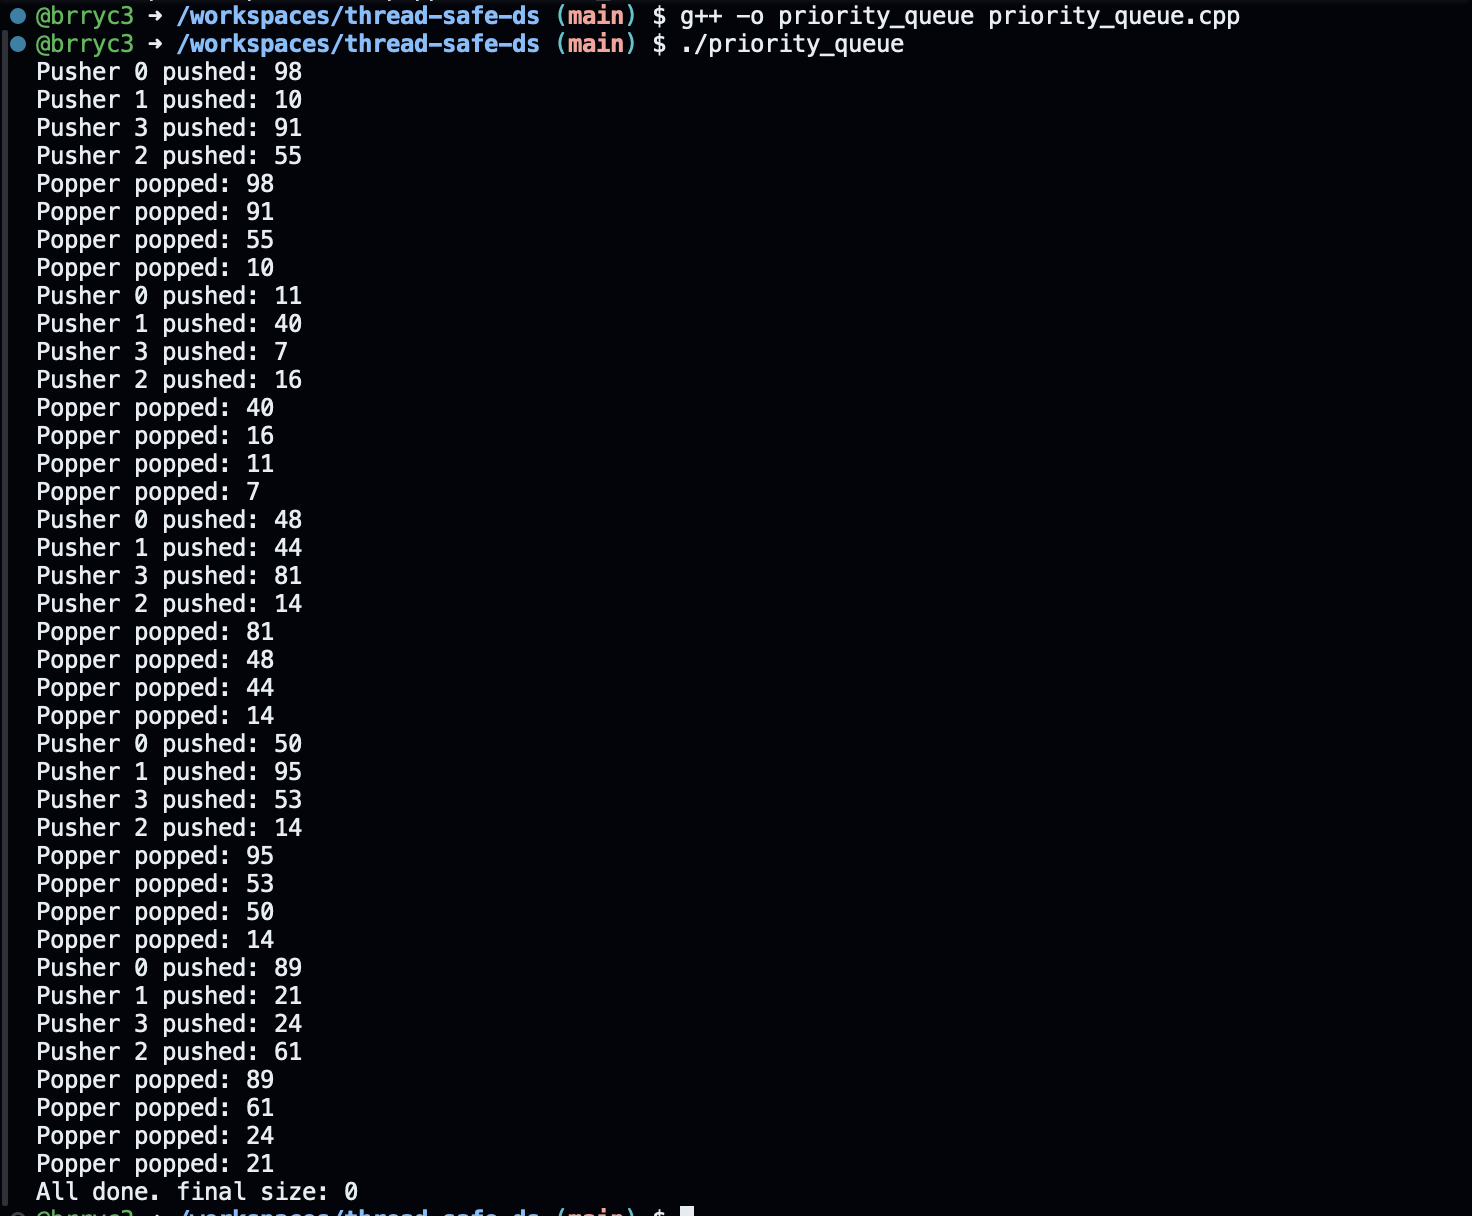
\includegraphics[width=\textwidth]{2_screenshot.png}
    \caption{Compilation and execution of priority_queue.cpp}
\end{figure}

\section{Exercise 4: Thread-Safe Circular Buffer}
\lstinputlisting[language=C++]{circular_buffer.cpp}

\textbf{Explanation}: Explain the use of condition variables for synchronization.

\textbf{Analysis}: Compare to ThreadSafeQueue from Exercise 1.

\textbf{Screenshot}: Include a screenshot of compiling and running circular_buffer.cpp.
\begin{figure}[h]
    \centering
    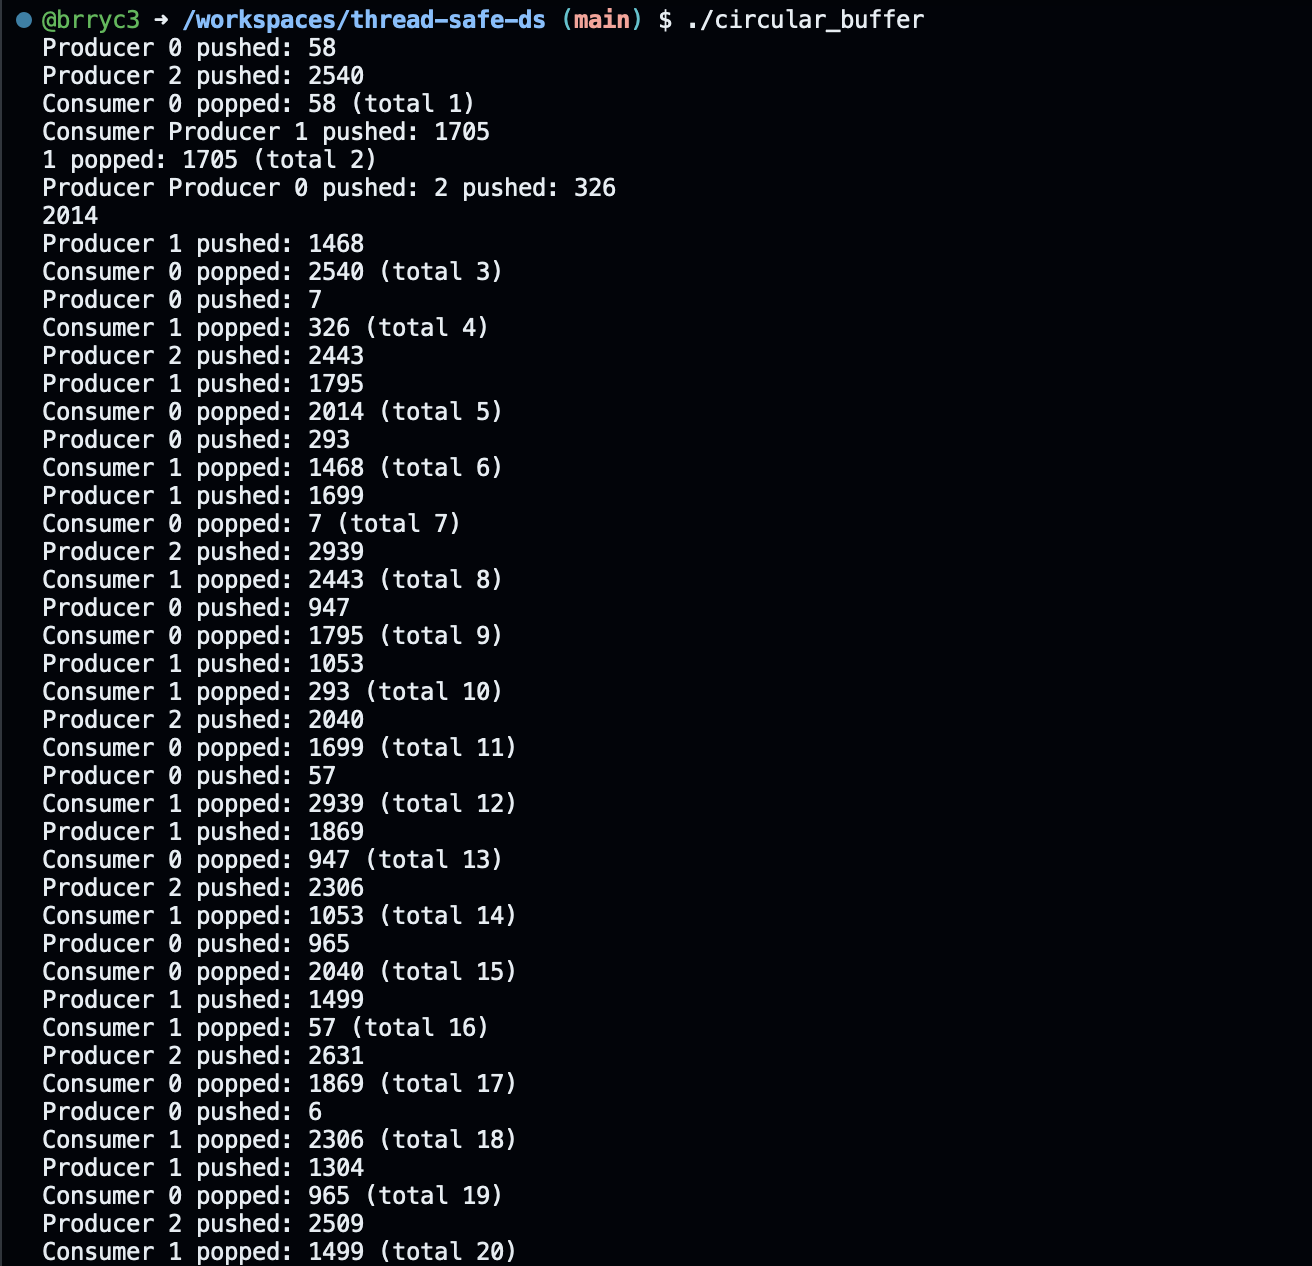
\includegraphics[width=\textwidth]{3_screenshot.png}
    \caption{Compilation and execution of circular_buffer.cpp}
\end{figure}

\section{Exercise 5: Thread-Safe Deque}
\lstinputlisting[language=C++]{thread_safe_deque.cpp}

\textbf{Explanation}: Describe the challenges of synchronizing access to both ends.

\textbf{Analysis}: Analyze concurrent operations on the deque.

\textbf{Screenshot}: Include a screenshot of compiling and running thread_safe_deque.cpp.
\begin{figure}[h]
    \centering
    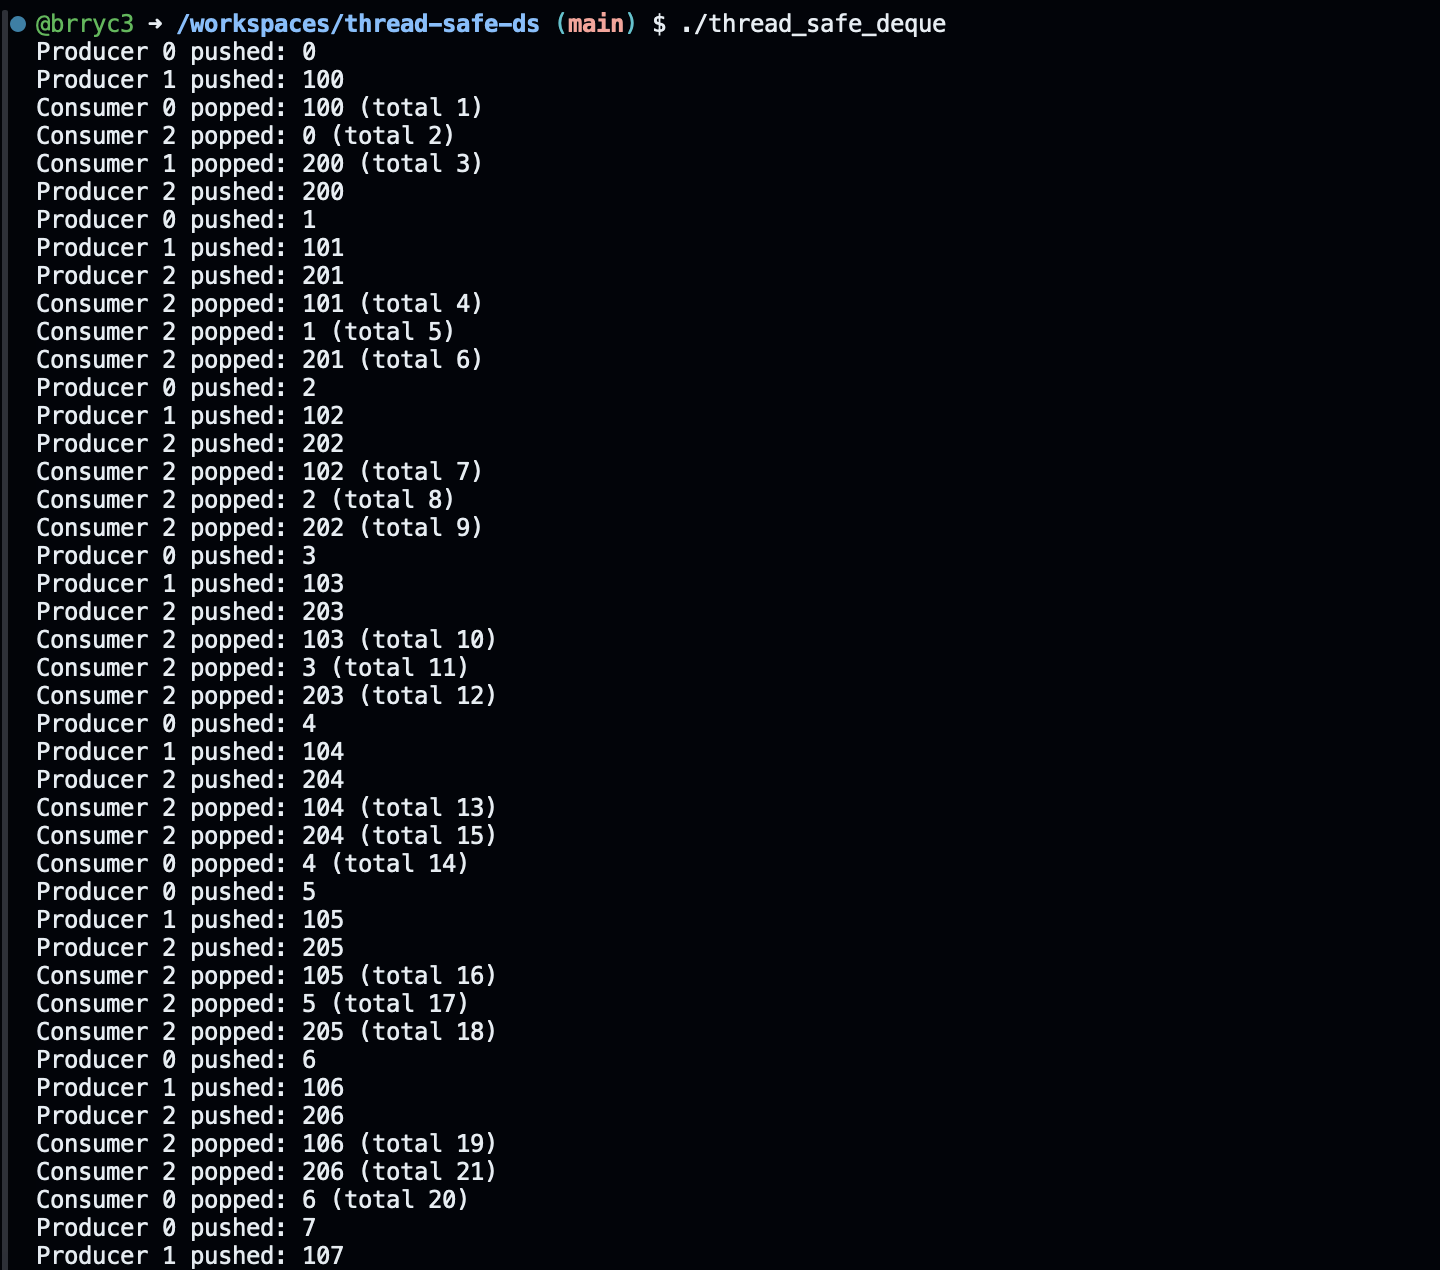
\includegraphics[width=\textwidth]{4_screenshot.png}
    \caption{Compilation and execution of thread_safe_deque.cpp}
\end{figure}

\section{Exercise 6: Thread-Safe Linked List}
\lstinputlisting[language=C++]{thread_safe_linked_list.cpp}

\textbf{Explanation}: Discuss maintaining list integrity during concurrent operations.

\textbf{Analysis}: Analyze thread safety and performance considerations.

\textbf{Screenshot}: Include a screenshot of compiling and running thread_safe_linked_list.cpp.
\begin{figure}[h]
    \centering
    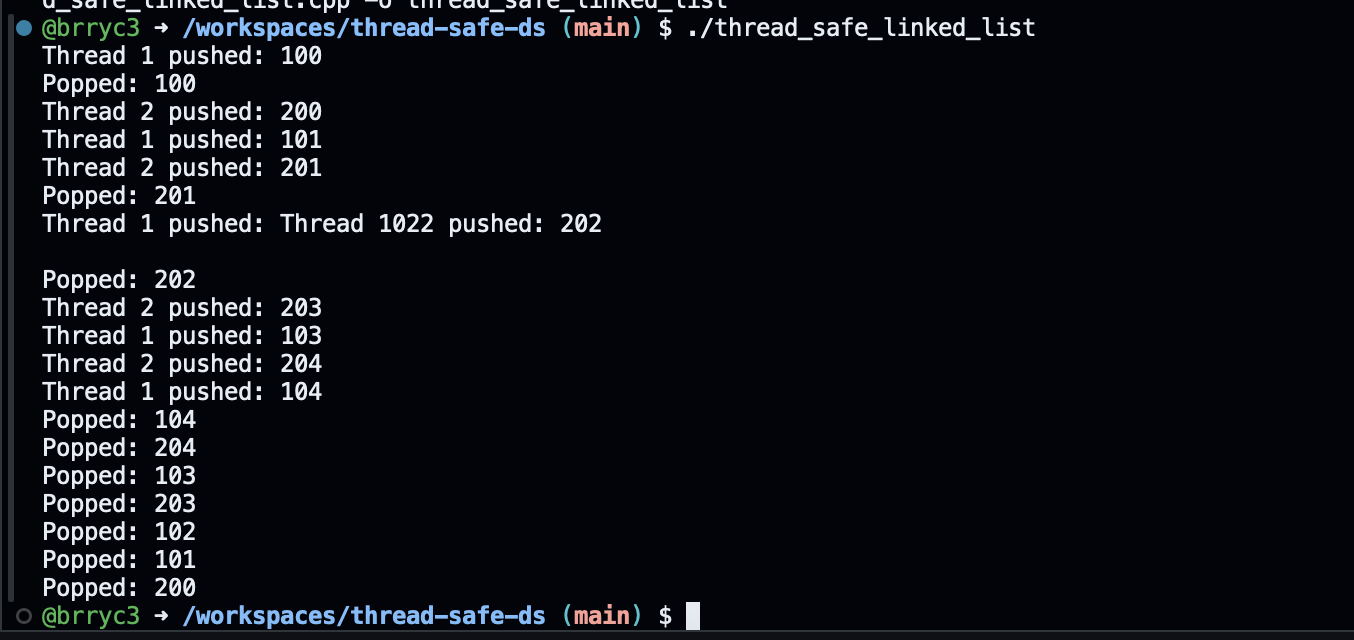
\includegraphics[width=\textwidth]{5_screenshot.png}
    \caption{Compilation and execution of thread_safe_linked_list.cpp}
\end{figure}

\end{document}